\section{O Som}
Diariamente somos expostos a diversas fontes sonoras, que podem nos afetar de maneira positiva ou negativa. Sons da chuva ou de músicas calmas trazem-nos alívio e sensação de descanso. Já o som de ambientes com muita conversa ou do tráfego intenso de veículos gera em nós desconforto e estresse. As ondas sonoras desempenham papel muito importante em nosso cotidiano e possuem características que podem nos auxiliar constantemente.

O som é uma onda mecânica (tipo de onda que precisa de um meio de propagação), tridimensional (propaga-se em todas as direções) e longitudinal (o tipo de vibração que gera é paralela à sua propagação). A imagem abaixo representa o esquema de uma onda sonora, mostrando-nos uma fonte sonora apontada para a direita, bem como as regiões de compressão e rarefação das moléculas de ar, o que caracteriza as ondas sonoras como longitudinais.

\begin{figure}[hb]
    \centering
    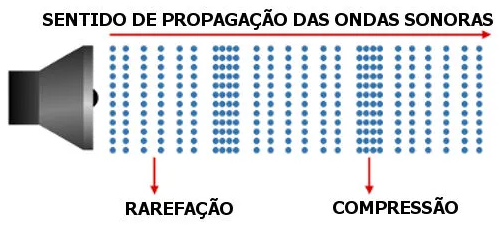
\includegraphics[width=0.6\textwidth]{imgs/propagacao_som.png}
    \caption{Propagação do Som}
    \label{fig:my_labeel}
\end{figure}

As ondas sonoras podem sofrer os fenômenos ondulatórios da reflexão, refração, difração e interferência.

Um exemplo de reflexão é o eco, que se caracteriza pela distinção entre o som produzido por uma fonte e o som refletido por um obstáculo. Como exemplo de refração dessas ondas, podemos citar a ocorrência de algo parecido com as miragens. Em dias quentes, em virtude da mudança no índice de refração do ar próximo a superfícies muito quentes, o som sofre desvios – esse fenômeno é dificilmente percebido. A difração, por sua vez, ocorre quando as ondas sonoras contornam obstáculos. Quando a porta de um ambiente está entreaberta, por exemplo, podemos ouvir o som produzido lá dentro. Finalmente, a interferência é um fenômeno decorrente do encontro de ondas sonoras produzidas por mais de uma fonte. Nesse contato, uma onda pode destruir a outra, a chamada interferência destrutiva, e gerar, mesmo em um ambiente barulhento, regiões de silêncio.

Existem propriedades relacionadas com a nossa capacidade de percepção do som que são denominadas de propriedades fisiológicas do som. O ouvido humano não consegue captar todas as frequências a que está exposto, mas existe um intervalo de frequências audível para os seres humanos, que varia aproximadamente de, no mínimo, 20 Hz a, no máximo, 20.000 Hz. Sons abaixo do mínimo percebido pelo sistema de audição humano são denominados de infrassons. Já os sons acima do máximo de captação são chamados de ultrassons. A tabela abaixo mostra os valores do espectro das ondas sonoras, indicando os intervalos de frequência para diferentes animais. Repare que sons que, por exemplo, são audíveis para os cães são considerados ultrassons para os humanos, isso porque estão além da capacidade de audição humana.


\begin{table}[hb]
\centering
\begin{tabular}{|cc|}
\hline
\multicolumn{2}{|l|}{Intervalo de frequências audíveis (Hz)}                           \\ \hline
\multicolumn{1}{|c|}{Humanos} & \multicolumn{1}{c|}{20 - 20.000} \\ \hline
\multicolumn{1}{|c|}{Cães} & \multicolumn{1}{c|}{15 - 50.000} \\ \hline
\multicolumn{1}{|c|}{Morcegos} & \multicolumn{1}{c|}{1000 - 12000} \\ \hline
\multicolumn{1}{|c|}{Golfinhos} & \multicolumn{1}{c|}{150 - 150000} \\ \hline
\end{tabular}

\caption{Intervalo de frequências audíveis} 
\end{table}

Existem aplicações tecnológicas para os sons que não somos capazes de ouvir. Uma delas é o diagnóstico por imagens feito a partir de ultrassons, os chamados exames de ultrassonografia. Nesse tipo de exame, ondas de alta frequência são direcionadas para órgãos ou fetos a serem analisados e, a partir da reflexão dessas ondas, um computador gera imagens. Os sonares, utilizados por submarinos, têm funcionamento semelhante ao do aparelho de ultrassom e mostram a distância e as dimensões de obstáculos à frente do submarino.

Outra propriedade física do som é a sua velocidade de propagação, que depende das características do meio no qual ocorre a propagação. Para a propagação do som em fluidos, a velocidade pode ser determinada a partir da equação abaixo, em que B é uma grandeza chamada de elasticidade volumar, que determina as características das substâncias ao serem comprimidas, e rho é a densidade do fluido.

$$
v= \sqrt{\frac{B}{\rho}}
$$
\begin{center}
    Equação 7 – Velocidade de propagação do som.
\end{center}

Repare que a densidade do fluido e a velocidade de propagação do som são inversamente proporcionais, pois, quanto mais denso é o meio, maior é a dificuldade de perturbação de suas partículas, o que dificulta a propagação e, por consequência, diminui a velocidade do som no meio.

A tabela abaixo indica o meio de propagação e a velocidade do som nesse meio em Km/h.

\begin{table}[hb]
\centering
\begin{tabular}{|c|c|}
\hline
\textbf{Meio de Propagação} & \textbf{Velocidade do som (Km/h)} \\ \hline
Ar                          & 12348                             \\ \hline
Hélio                       & 34992                             \\ \hline
Água                        & 5328                              \\ \hline
Mercúrio                    & 5220                              \\ \hline
Borracha                    & 194,4                             \\ \hline
Chumbo                      & 4680                              \\ \hline
Ouro                        & 11664                             \\ \hline
Aço                         & 21384                             \\ \hline
Diamante                    & 43200                             \\ \hline
\end{tabular}
\caption{Meio de propagação e a velocidade do som nesse meio em Km/h.}
\end{table}

Por fim, a intensidade pode ser citada como uma importante propriedade do som. Qualquer movimento ondulatório transporta energia, portanto, se uma onda sonora atravessar uma determinada área em certo intervalo de tempo, a energia carregada por ela também atingirá essa área. A energia transportada pelo som é que faz o corpo tremer, por exemplo, diante do som produzido em um show musical. Assim sendo, a intensidade sonora é a determinação dessa quantidade de energia que atravessa uma área em determinado intervalo de tempo e pode ser calculada a partir da seguinte expressão:

$$
I = \frac{\Delta E}{A\cdot \Delta t}
$$

\begin{center}
    Equação 8 – Intensidade sonora.
\end{center}

A razão entre energia e tempo é definida como potência. Assim, podemos reescrever a equação como:

$$
I = \frac{P}{A}
$$
\begin{center}
    Equação 9 – Equação anterior reescrita.
\end{center}

A unidade de medida da intensidade sonora no Sistema Internacional de Unidades é o W/m2.

Para medir a sensação que o som produz ao atingir nosso aparelho auditivo, temos uma grandeza chamada de nível de intensidade sonora, que está expressa a seguir.

$$
\beta = \log\left ( \frac{I}{I_{0}} \right )
$$
\begin{center}
    Equação 10 – Nível de intensidade sonora
\end{center}

Nessa equação, I0 é a mínima intensidade sonora percebida pelo ouvido humano e vale 10 –12 W/m2. A unidade de medida do nível sonoro é o bel (B), isso em homenagem ao inglês Graham Bell, inventor do telefone. Mas a unidade utilizada é uma fração do bel, definida como decibel (dB). A tabela abaixo traz o nível sonoro para distintas fontes.

\begin{table}[hb]
\centering
\begin{tabular}{|cc|}
\hline
\multicolumn{2}{|c|}{\textbf{Níveis de intensidade sonora}}       \\ \hline
\multicolumn{1}{|c|}{\textbf{Fonte sonora}} & \textbf{Nível (dB)} \\ \hline
\multicolumn{1}{|c|}{Próxima a um jato}     & 150                 \\ \hline
\multicolumn{1}{|c|}{Limiar da dor}         & 120                 \\ \hline
\multicolumn{1}{|c|}{Sirene}                & 110                 \\ \hline
\multicolumn{1}{|c|}{Aspirador de pó}       & 80                  \\ \hline
\multicolumn{1}{|c|}{Mosca}                 & 40                  \\ \hline
\end{tabular}
\caption{Nível sonoro}
\end{table}

Como exemplo de aplicação do cálculo da intensidade de ondas, podemos citar a Escala Richter, desenvolvida em 1935 por Charles Francis Richter e Beno Gutenberg. Essa escala determina a energia sísmica liberada durante um terremoto.

Os sons desempenham papel fundamental em nosso cotidiano e fazem parte do ramo da Física chamado de Ondulatória, responsável pelo estudo das ondas.